\begin{refsection}
    \renewcommand{\thefigure}{\arabic{figure}}
    
    \chapter[``Vencido o {\itshape New Look}'': {\itshape resistências femininas a Christian Dior e as suas modas (Natal/RN, 1948--1953)}]{``VENCIDO O {\itshape NEW LOOK}\footnote{Em tradução literal, \textit{new look} significa ``novo olhar'', tal termo foi designado por Carmel Snow, repórter norte-americana da revista Vogue, quando foi cobrir a coleção de lançamento da marca Dior. Termo que será abordado de forma mais profunda no decorrer do trabalho.}''\\Resistências femininas a Christian Dior e as suas modas (Natal/RN, 1948--1953)}

    \label{chap:vencidonewlook}
    
    \articleAuthor
    {João Vieira Neto}
    {Discente do curso de Licenciatura em História. Bolsista IC/Propesp/UFRN. ID Lattes: 9127.3680.8474.7839. ORCID: 0000-0001-7244-4573. E-mail: jvieiran00@gmail.com.}

    \articleAuthor
    {Joel Carlos de Souza Andrade}
    {Professor do Departamento de História/CERES/UFRN e do Mestrado em História dos Sertões/UFRN. ID Lattes: 6752.7281.1456.8336. ORCID: 0000-0003-2141-0212. E-mail: jocadesoan@yahoo.com.br.}
    
    \begin{galoResumo}
        \marginpar{
            \begin{flushleft}
            \tiny \sffamily
            Como referenciar?\\\fullcite{SelfVieiraNetoAndAndrade2021}\mybibexclude{SelfVieiraNetoAndAndrade2021}, p. \pageref{chap:vencidonewlook}--\pageref{chap:vencidonewlookend}, \journalPubDate{}
            \end{flushleft}
        }
        Discute o estilo \textit{``new look''} desenhado pelo estilista francês Christian Dior em 1947, e como este foi apropriado e criticado pelas moças em Natal durante os anos de 1948--1953, a partir do periódico potiguar \textit{Diário de Natal}. No caso do francês, suas reportagens destacaram a sua ousadia em relação à criação visto que a situação mundial estava desfavorável à moda em virtude da economia fragilizada, causada pela Segunda Guerra Mundial. Entretanto, as intempéries econômicas não foram suficientes para que Dior suspendesse suas criações, e apresentasse uma nova silhueta, a qual acentuava a feminilidade. Entre as notícias, é possível perceber resistências através do discurso jornalístico, devido os problemas econômicos. Metodologicamente, o estudo constitui-se a partir de consultas ao \textit{Diário de Natal}, e análise de autores como Gilles Lipovetsky (1989), Medeiros Filho (2014) e Luca (2009), essenciais para a tessitura do estudo em questão. As informações sobre a moda feminina eram refletidas entre 1948--1950 no periódico na seção ``Notícias da Moda'' e expunha notícias acerca do modismo vigente, marcado pela criação de Christian Dior. A despeito do descontamento das natalenses, no contexto pós Segunda Guerra Mundial, as criações do estilista não foram interrompidas e bem como suas apropriações por tais moças resistentes.
    \end{galoResumo}
    
    \galoPalavrasChave{Imprensa. História da Moda. Cidade do Natal.}

    \filbreak

    \begin{otherlanguage}{english}

    \fakeChapterTwoLines
    {The \textit{New Look} vanquished}
    {women's resistance to Christian Dior and his fashions (Natal/RN, 1948--1953)}

    \begin{galoResumo}[Abstract]
        It discusses the ``new look'' style designed by the French designer Christian Dior in 1947, and how it was appropriated and criticized by the girls in Natal during the years 1948--1953, from the Rio Grande do Norte newspaper \textit{Diário de Natal}. In the case of the French, his reports highlighted his boldness in relation to creation, since the world situation was unfavorable to fashion due to the fragile economy, caused by the Second World War. However, the economic maelstrom was not enough for Dior to suspend his creations, and to present a new silhouette, which accentuated femininity. Among the news, it is possible to perceive resistance through the journalistic discourse, due to economic problems. Methodologically, the study is constituted by consultations with the \textit{Diário de Natal}, and analysis of authors such as Gilles Lipovetsky (1989), Medeiros Filho (2014) and Luca (2009), who are essential for the design of the study in question. Information about women's fashion was reflected between 1948--1950 in the newspaper, at the section ``Notícias da Moda'' (News of Fashion), which exposed news about the fad of the time, marked by the creation of Christian Dior. Despite the Natalense discontent, in the post-World War II context, the stylist's creations were not interrupted and neither were his appropriations by such resistant girls. 
    \end{galoResumo}
    
    \galoPalavrasChave[Keywords]{Press. History of Fashion. City of Natal.}
    \end{otherlanguage}

    \section[Riscando o croqui, riscando uma introdução]{Riscando o croqui\footnote{Termo utilizado para referir-se a desenho, molde.}, riscando uma introdução}

    ``Nos trajes, posturas e gostos se encontram em uma interface entre os mais variados elementos simbólicos que edificam as sociedades'' \cite[p.~14]{SilvaMonteleoneDebom2019HistoriaModa}. A partir deste fragmento, constante no livro \textit{A história na moda, a moda na história}, os autores expressaram uma característica acerca do estudo das vestes: o estudo das sociedades por meio do trabalho com as roupas, os fios dos tecidos culturais, econômicos e sociais encontram-se na teia que configura a pesquisa com a roupa e a moda.  

    Neste sentido, \textcite{Calanca2008Historia} argumenta que a ``moda é oposta ao costume visto que a primeira se configura enquanto conflito temporal, do antigo e do contemporâneo, pela inconstância, ao passo que o costume é marcado pela perpetuação, pela continuidade: alude numa primeira instância, a uma dicotomia temporal entre o `velho' e o `novo', entre o presente e o passado, entre imobilidade e mobilidade'' \cite[p.~11]{Calanca2008Historia}. Através das concepções da autora citadas anteriormente percebe-se que o sistema da moda se encontra imerso em uma dicotomia, um embate entre a tradição e a efemeridade, assim, os enfrentamentos concernentes ao \textit{new look} perpassam também por essas questões temporais.  

    Compreendida enquanto sistema, logo, compreendida pela perspectiva histórica, a moda floresceu durante o Renascimento entre as décadas de 1340 e 1350, de acordo com Gilles \textcite{Lipovetsky1989Imperio}. Em seu livro \textit{O Império do Efêmero: a moda e os seus destinos na sociedade moderna}, o filósofo expõe que tal sistema surgiu na Europa moderna a partir da oposição entre os burgueses mais jovens e os mais velhos, enquanto sistema econômico, social e, sobretudo, cultural. Ainda que, segundo o autor, ``a questão da moda não faz furor no mundo intelectual'' \cite[p.~13]{Lipovetsky1989Imperio} a moda é passível de ser objeto de estudo, da Sociologia, Economia, Filosofia, Antropologia, do Direito e da História, como no presente estudo. Em nossa contemporaneidade, como argumenta a historiadora Maria do Carmo Teixeira \textcite{Rainho2015Moda}, as pesquisas em moda, na perspectiva histórica, cresceram a partir dos cursos superiores na área de moda, bem como os programas de pós-graduação. Talvez, a moda esteja fazendo furor no mundo intelectual, contradizendo o que afirmara Lipovetsky à época em que publicara o seu trabalho.

    Assim, enquanto fonte histórica, a moda permite o conhecimento de sociedades anteriores, as culturas dominantes e dominadas, bem como as formas que os indivíduos tensionavam socialmente para se destacarem socialmente por meio de seus trajes, permite identificar as reminiscências das roupas passadas, as quais ainda se fazem presentes e se perpetuam na contemporaneidade. Logo, nada mais contemporâneo do que a moda, conforme afirma Giorgio Agamben, pois ``aquilo que define a moda é que ela introduz no tempo uma peculiar descontinuidade que o divide segundo a sua atualidade ou inatualidade, o seu estar ou o seu não-estar-mais-na-moda'' \citeyear[p.~66]{Agamben2009Conteporaneo}.

    Através de Agamben, entende-se que a contemporaneidade se materializa na moda, em virtude de (des)ordem temporal que a mesma instaurou desde o seu florescer no Renascimento, no caso do \textit{new look}, a revolução se deu em virtude da transformação da silhueta feminina, aspecto que ainda será tratado neste trabalho.

    Considerando o caráter de fonte, que a moda performa, somou-se ao \textit{corpus} documental a pesquisa em periódicos, mais especificamente o jornal potiguar \textit{Diário de Natal}, veículo de imprensa a principal ferramenta para a tessitura do presente estudo. Para tanto, Tânia Regina de Luca problematiza, em \textit{História dos nos, e por meio dos periódicos}, as questões relacionadas ao trato com as fontes hemerográficas. Estes registros são recentes para o uso da História visto que sua exploração se iniciara na década de 1970, sofrendo resistências em virtude da subjetividade dos jornais, dos seus discursos tendenciosos, e sobretudo os seus silêncios. É que antes da virada historiográfica da década de 1970, os historiadores preocupavam-se essencialmente com a verdade, a qual estava presente somente nos documentos ditos oficiais.

    Entretanto, apesar das resistências que os jornais e revistas sofreram para serem utilizados pelos historiadores, de Luca ressalta que ``a ênfase em certos temas, a linguagem e a natureza do conteúdo tampouco se dissociam do público que o jornal ou revista pretende atingir'' \cite[p.~140]{Luca2009Historia}. A partir de tal consideração, uma característica marcante da imprensa, a qual relaciona-se diretamente com as proposições desta pesquisa, concerne ao direcionamento dos discursos produzidos por jornais, para estratos sociais específicos, neste caso em especial, às leitoras do \textit{Diário de Natal}, entre os anos de 1948--1953. Nesta pesquisa, o periódico retratava as modas, noticiava as natalenses sobre as tendências estrangeiras assim como corroboravam nas resistências que as parisienses, novaiorquinas e cariocas tinham ao \textit{new look}, tais concepções agiam diretamente no imaginário das natalenses --- que tanto resistiam quanto consumiam tais modas.

    Desta forma, através dos discursos jornalísticos dotados de subjetividade, insere-se uma das problemáticas que permeiam o presente estudo: como tais discursos performavam-se no jornal analisado, tendo em vista que o caráter do \textit{Diário de Natal} era de ser um jornal político, mas ainda assim temáticas como moda se fizeram presentes. Por meio desta perspectiva política, a pesquisa deste periódico tornou-se mais complexa visto que o enfoque do \textit{Diário de Natal} era trabalhar em sua maioria com acontecimentos políticos, enaltecendo as realizações de grandes homens, considerados importantes para a história do Rio Grande do Norte. Uma peculiaridade também desta pesquisa, pois volta os seus olhares e interesses para tecer uma outra história de Natal e do Rio Grande do Norte, não preocupada no positivismo falocêntrico, mas tendo outras prioridades (moda, resistência) e apresentando outras possibilidades para a historiografia potiguar.  

    Deste modo, o presente estudo enveredar-se-á pelas casas de costura francesas, exaltando como as modas eram apropriadas ao passo que eram rejeitadas pelas moças, em um movimento de apatia externa a qual desembocava internamente e influenciava as natalenses em suas formas de se apresentar publicamente. Ainda que o trabalho em questão, enquanto um \textit{patchwork}\footnote{De acordo com o Dicionário online de português, \textit{patchwork} performa-se enquanto tecido com retalhos, no sentido deste trabalho, assume a definição de elementos díspares que se combinam, logo, moda, jornais e o Rio Grande do Norte.}, constrói-se por meio das fontes hemerográficas, não é considerado um estudo sobre imprensa de moda, pois, como citado anteriormente, o caráter do periódico analisado era político. A delimitação temporal ocorreu a partir das primeiras ocorrências do \textit{Diário de Natal} (disponíveis na Hemeroteca Digital), no ano de 1948, enquanto marco inicial, ainda que o modelo \textit{new look} houvesse sido desenhado no ano anterior, em 1947, e como marco final o ano de 1953, pois foram quando as últimas ocorrências sobre o costureiro e estilista francês Christian Dior apareceram no periódico.

    Mesmo que o \textit{new look} houvesse sido criado em 1947, marcando a década de 1950 como a silhueta clássica, tal tendência transcendeu os limites dos ``anos de ouro'' e permaneceu nas décadas posteriores, assinalando a importância de Dior e de sua \textit{maison}\footnote{\textit{Maison}, termo em francês para referir-se à casa. No tocante à \textit{maison} Dior, equivale-se à casa de costura do estilista francês.} na indústria e na história da moda.

    Tal enfoque se apresenta como relevante para a historiografia potiguar, tendo em vista a carência em estudos históricos sobre as vestes, o costurar e suas relações de apropriação e releituras face aos costumes da sociedade. Portanto, a despeito de ser uma reflexão inicial, esta abordagem aponta para a relevância e riqueza históricas destes estudos no âmbito de uma história da moda.

    Como forma de aprimorar a compreensão acerca das temáticas que serviram de tema para a tessitura do trabalho em questão, o mesmo será fragmentado em seções menores: ``Christian Dior pelas páginas natalenses'', a qual abordaremos a presença do francês entre os anos analisados, percebendo principalmente a resistência feminina atrelada a ele e às suas criações; ``New Look: revolução e resistência'', onde compreenderemos como o \textit{new look} foi representado no \textit{Diário de Natal}, principalmente a divergência de opiniões femininas frente ao modelo em questão e ao sistema da moda, em virtude da situação econômica acometida pelos conflitos armados da Segunda Guerra Mundial, uma tendência que estava entre a recusa e a sedução das moças natalenses; e ``Notícias da Moda, uma seção de modos e modas'', por meio da análise de tal fragmento do jornal, identificaremos como a seção ``Notícias da Moda'' era responsável não somente por apresentar as tendências dominantes e que surgiam na indústria da moda, mas principalmente os discursos desta seção atrelados às roupas e ao comportamento feminino, como tal parte do jornal conseguia moldar o imaginário das natalenses entre os anos de 1948--1953, haja vista a capacidade formativa e informativa dos jornais daquela época.

    \section{Christian Dior pelas páginas natalenses}

    O cerne desta exposição não é debruçar-se sobre a vida e obra de Christian Dior, mas explorar a sua principal criação, e como esta foi apropriada e, sobretudo, recusada pelas natalenses entre o fim da década de 1940 e início da de 1950, entretanto, consideramos válida uma breve contextualização acerca do estilista para que os reflexos dele e do \textit{new look} na imprensa natalense, tornassem-se mais explícitos e compreensíveis.  

    Em sua dissertação de mestrado, intitulada \textit{Arremedando Dior: a moda do New Look em São João do Sabugi-RN (anos 1950)}, \textcite{MedeirosFl2014Arremedando} argumenta que Christian Dior era natural de Granville na Normandia, nasceu em 1905, numa família burguesa, desde criança havia despertado para o desenho, sobretudo o de máscaras, estudou Ciências Políticas em Paris, ainda que tivesse o desejo de cursar Belas Artes. Ao chegar na ``capital da moda'', não obteve êxito com a política e, para sobreviver, decidiu trabalhar com moda. Passou a desenhar e vender \textit{croquis} para jornais parisienses, até que conseguiu notoriedade e foi contratado por Robert Piguet, para o seu ateliê, em seguida, trabalhou para o também modista Lucien Lelong até que conseguiu que Marcel Boussac financiasse a abertura de sua casa de moda.  

    Embora estivesse entre os modistas e os comerciantes de tecidos, a inserção de Christian Dior na indústria da moda não foi fácil, principalmente quando lançou a sua coleção de estreia em 1947, em virtude dos problemas econômicos sofridos pela França do pós guerra. Segundo Medeiros Filho, ``a entrada de Dior no restrito círculo dos criadores de moda na capital francesa deu-se com o choque da invenção de um estilo espalhafatoso, contrário às tendências restritivas que vigoravam desde a Segunda Guerra Mundial'' \citeyear[p.~115]{MedeirosFl2014Arremedando}.

    Por meio da citação, percebemos que Dior emergiu enquanto um revolucionário da moda, o qual abandonou o estilo sóbrio e simplificado, para instaurar uma nova ordem estética, a ordem do exagero, refletida nas amplas e rodadas saias que compuseram o \textit{new look}.

    \begin{quotation}
        Dior surpreendeu o mundo em 1947, lançando sua primeira coleção de moda, inicialmente chamada Linha Corola, depois apelidada New Look. A grande tendência que apresentou era a de uma exagerada forma feminina, em que a silhueta era construída artificialmente através de gasto extravagante de tecido \cite[p.~115]{MedeirosFl2014Arremedando}. 
    \end{quotation}

    Identificamos que Christian Dior, como costureiro e estilista, apresentou-se para a sociedade parisiense bem como para a indústria da moda, enquanto um revolucionário do estilo, revolucionário das formas estéticas, bem como que o nome da coleção de lançamento não era \textit{New Look}, e sim Linha Corola. Entretanto, mediante o sucesso daquela tendência a partir da publicidade de moda, por jornais e principalmente revistas de moda, não somente as francesas, mas sobretudo as estadunidenses como a Vogue. Neste sentido, \textcite{Crane2006Moda} nos ajuda a pensar acerca da disseminação da moda por meio desses veículos midiáticos pois as consumidoras da moda poderiam ter acesso àquelas roupas, àquelas modas, ainda que não vestissem necessariamente um modelo de Dior.

    A autora em questão, em \textit{A moda e seu papel social: classe, gênero e identidade das roupas}, ainda revela que Dior é considerado fundamental para a indústria da moda em virtude da propagação da sua \textit{maison}, por meio do perfume. Segundo Crane, no período posterior à Segunda Guerra Mundial, as \textit{maisons} de alta-costura francesas passaram por momentos delicados, em virtude da contenção de gastos com futilidades como roupas e sapatos, e principalmente devido à uma nova tendência que crescia e tornava-se oposta à alta-costura, que era o \textit{prêt-à-porter}\footnote{Produção em série de roupas, comercializadas em lojas. Não eram consideradas objetos artísticos, como as roupas de alta-costura. Eram peças mais simplificadas, ainda que acompanhassem a moda.}. Por meio do \textit{prêt-à-porter}, um segmento crescente na indústria da moda, a alta-costura precisou reinventar-se frente não somente à competição, mas com o risco de desaparecer. Face ao novo desafio, uma alternativa amplamente usada pela \textit{maison} Dior foi o licenciamento de produtos, como considera Crane:

    \begin{quotation}
        A principal fonte de renda das empresas anteriores à guerra que sobreviveram, bem como das novas empresas que entraram no mercado depois dessa época foram os \textit{royalties}\footnote{8} obtidos pelo licenciamento de uma diversidade produtos, que iam de roupas a aparelhos domésticos \citeyear[p.~286]{Crane2006Moda}.
    \end{quotation}

    Deste modo, compreendemos que Dior, para além do costureiro e estilista que revolucionou a moda e a silhueta feminina, assinalando o estilo clássico dos anos 1950, era também uma marca e principalmente um produto que gerava lucro por meio do comércio de itens que carregavam consigo a patente ou a marca Dior. Crane ressalta que a \textit{maison} Dior que era uma marca de alta-costura, frente às intempéries econômicas ocasionadas pela Segunda Guerra Mundial que passou a produzir também os seus itens de \textit{prêt-à-porter}.

    Pelas páginas natalenses, o estilista Christian Dior foi retratado a partir das suas criações, como grandes brincos com correntes e pedras coloridas, atrelado a grandes nomes da alta-costura, como Pierre Balmain, onde apareciam enquanto lançadores de tendências extravagantes e exóticas, advindas de Paris que terminavam por desembocar em Natal. Deste modo, é possível perceber as relações estabelecidas entre o sistema da moda e as diferentes localizações. Dior ainda apareceu relacionado ao desfile promovido pelo Museu de Arte de São Paulo (MASP) em 1952, por Pietro Maria Bardi, o qual importou da França a coleção daquele ano da \textit{maison} Dior para o evento que inauguraria a seção de costumes do museu.

    Segundo o periódico, Christian Dior presenciou o baile promovido pelo também estilista francês Jacques Fath. Este havia se inspirado no carnaval brasileiro e apresentou na ocasião modelos produzidos a partir do algodão Seridó, iniciativas promovidas pelo jornalista Assis Chateaubriand com o claro objetivo de integralizar o ``ouro branco'' potiguar ao resto do Brasil e do mundo. Na reportagem intitulada ``\citetitle{Chateaubriand1952Show}'', de Chateaubriand, Dior apareceu atrelado ao evento de tamanha importância para a moda francesa, mas o que chama mais atenção é que aquele estilista já havia utilizado o algodão seridoense, conforme relata o jornalista: ``É que ali se vão apresentar, pela primeira vez, na Europa, os tecidos brasileiros do algodão de fibra longa do Nordeste. A primeira tentativa se fez com o costureiro Christian Dior, faz dois anos''. Enquanto Fath estaria estrando publicamente a fibra do mocó, Dior já a tinha usado em 1950, e aparentemente não apresentou suas criações.

    Pelas ocorrências relativas a Christian Dior, o jornal apresenta silêncios no tocante à sua vida particular. Dior conseguiu seu destaque na indústria da moda por remodelar as formas femininas, excluindo os cortes mais sérios das vestes das damas, contudo, ainda que o estilista tivesse reformado a silhueta feminina durante a década de 1950, as moças mostraram-se apáticas e resistentes às suas modas, logo, a partir destas resistências que o trabalho em questão se construiu. Deste modo, considerou-se pertinente a contextualização das ocorrências acerca do costureiro para o presente estudo, visto que permitiu compreender o seu lugar de destaque na sociedade parisiense, bem como os elos entre Paris e Natal, como no caso em tela. Posteriormente, as matérias relacionadas ao estilista passaram a serem referentes às oposições femininas frente às modas produzidas pela \textit{maison} Dior. Assim, o \textit{new look} estava imerso em uma dubiedade, entre a revolução estética, da silhueta feminina e a resistência das mulheres no tocante aos novos modos de se apresentar em público.

    \section{\textit{New Look}, revolução e resistência}

    Trabalhar com o \textit{new look} tornou-se uma possibilidade de perceber a dubiedade entre a revolução e a resistência. Revolução, pois quando Christian Dior desenhou o seu modelo, em 1947, transformou a silhueta feminina, que até aquela altura era masculinizada. Em virtude dos problemas ocasionados pela 2ª Guerra Mundial e tal conflito demandava capital exclusivo para suprir suas dependências, e não havia espaço para o exagero com roupas e superficialidades, como argumenta Medeiros Filho: ``sobriedade e praticidade são palavras de ordem na busca do vestuário feminino adequado durante os tempos nebulosos da presença alemã em solo francês, com o fim dos exageros nos vestidos, nos acessórios e até na pintura das unhas e do rosto'' \cite[p.~103]{MedeirosFl2014Arremedando}. Logo, conforme pondera este historiador, o sistema de moda estaria consequentemente fadado ao fracasso, ou ao menos ao esquecimento, durante os primeiros anos posteriores ao conflito armado.

    Ainda que as situações econômica e social estivessem comprometidas, o costureiro e estilista não mediu esforços para revolucionar a indústria da moda, apresentando uma nova silhueta, abandonando as formas masculinas e retas, e adotando saias amplas, rodadas, peguilhadas, combinadas ao \textit{tailleur}\footnote{Conjunto de casaco e saia, ajustado à cintura, adaptado do vestuário masculino para a mulher. \cite[p.~229]{MedeirosFl2014Arremedando}.}, como na imagem a seguir (figura \ref{fig:new-look}).

    \begin{figure}[ht]%
        \centering%
        \caption{\textit{New Look}}%
        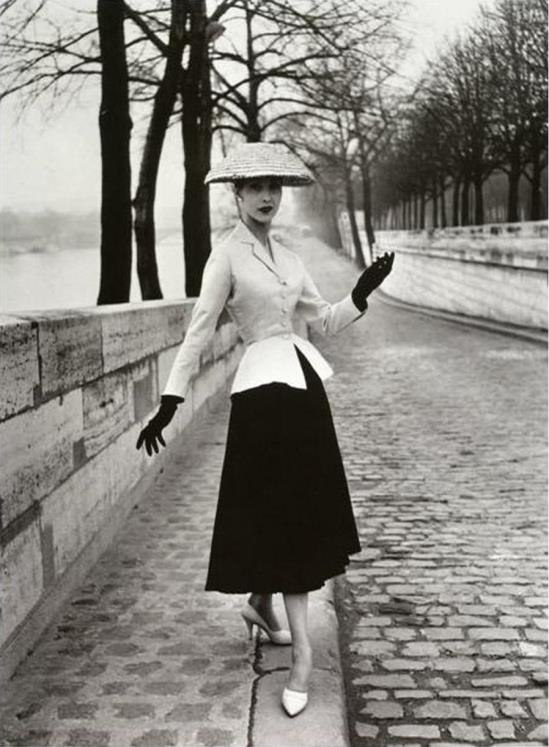
\includegraphics[width=.333\textwidth]{articles/06-vencido-o-new-look-r/01-new-look.jpg}%
        \caption*{Fonte: \textapud[p.~20]{Pochna2000Dior}[p.~58]{MedeirosFl2014Arremedando}.\mybibexclude{Pochna2000Dior}}%
        \label{fig:new-look}%
    \end{figure}%

    Através da imagem acima, percebe-se as características do \textit{new look}: cintura fina e marcada, ancas largas, saia comprida e rodada e chapéu complementar. De acordo com \textcite{MedeirosFl2014Arremedando}, o \textit{new look} foi o primeiro modelo a tomar proporções mundiais, o que se confirma quando se analisa periódicos como os que circularam no estado do Rio Grande do Norte, como o \textit{Diário de Natal}, fotografias do período e até mesmo revistas que não desembocavam nas localidades mais remotas, a exemplo da revista \textit{O Cruzeiro}, também fonte para este estudo.

    Neste sentido, a tendência que transcendeu a década de 1950 e repercutiu em temporalidades posteriores, como a década de 1960, com algumas variações, era formado por:

    \begin{quotation}
        \noindent{}os corpetes eram armados com barbatanas e, a partir de cinturas muito justas, abriam-se amplas saias, lembrando as corolas das flores. As saias poderiam ser pregueadas, franzidas, drapeadas ou nesgadas, sempre forradas com tule para darem o efeito de armação, resultando na forma corolácea de uma cúpula \cite[p.~116]{MedeirosFl2014Arremedando}.
    \end{quotation}

    Portanto, através das palavras de Medeiros Filho infere-se que a coleção tinha inspiração nas corolas de flores, prezando pela demarcação das formas femininas a partir de corpetes e quadris apertados, os quais definiam o ideal corpóreo das mulheres, em consonância com a inspiração de Dior que rememorava o século XIX, sobretudo com as anquinhas usadas por baixo das saias rodadas. 

    \begin{wrapfigure}{o}[\dimexpr \marginparsep+\marginparwidth]{0pt}%
        \begin{minipage}[b]{\marginparwidth}
            \caption{Reportagem ``Os modistas francezes de\-cre\-tam a morte do `New Look' e lançam o `New New'{}''.}
            \caption*{Fonte: Biblioteca Nacional, Brasil (Hemeroteca Digital) --- Diário de Natal, ano 1948, ed. 01658, 26 set. 1948.}
            \label{fig:morte-new-look}
        \end{minipage}
        \hspace{\marginparsep}
        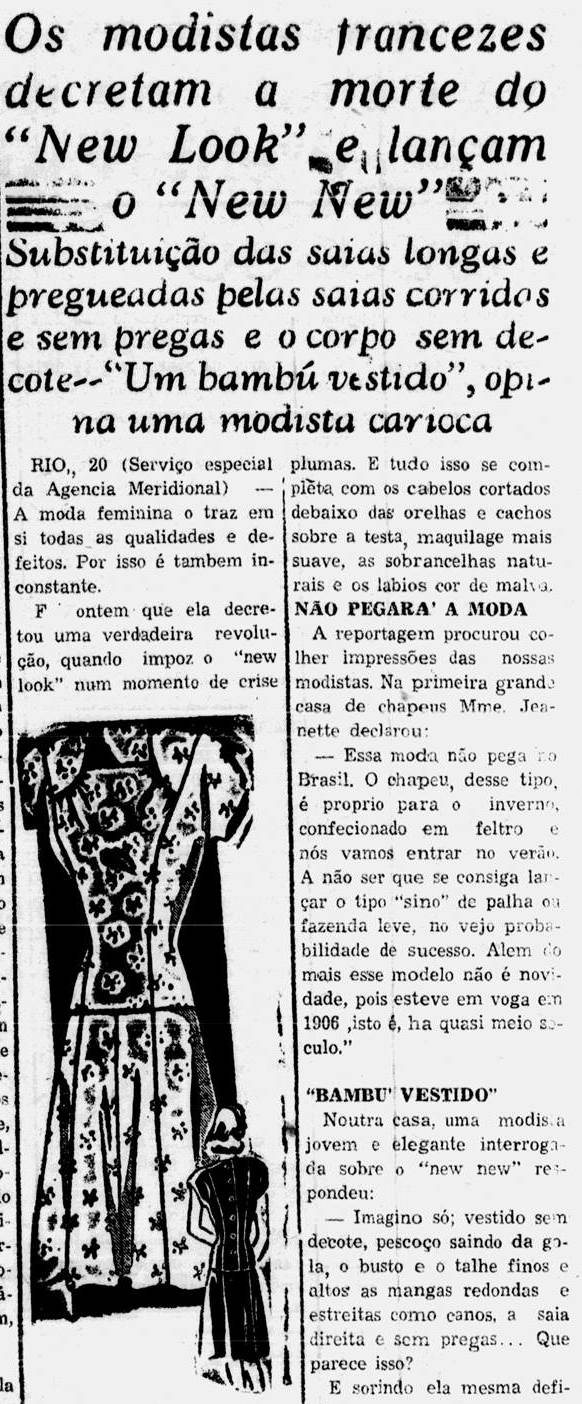
\includegraphics[height=25\baselineskip]{articles/06-vencido-o-new-look-r/02-morte-new-look.jpg}
    \end{wrapfigure}%

    \nocite{ModistasFrancezes1948}

    Deste modo, ainda que houvesse revolucionado não somente as formas estéticas, Dior conseguiu transformar o sistema da moda. Em consonância, a partir do \textit{new look} conseguiu inimigos, resistentes não apenas às suas modas escandalosas, rodadas e exacerbadamente femininas, mas resistentes a pessoa de Christian Dior, como faz refletir o título do presente texto ``resistências femininas a Christian Dior e as suas modas'', como foi percebida pelo jornal \textit{Diário de Natal}. Tratando-se das resistências, o jornal apresenta principalmente acerca dos problemas econômicos, questão trabalhada a seguir.  

    Entre as páginas natalenses, apre\-sen\-ta\-ram-se as mais diversas explicações para que as mulheres não adotassem o novo estilo, influenciadas pelas moças de Paris, de Nova York e do Rio de Janeiro. Dentre os motivos, o clima e as condições climáticas do Brasil. Chamou a atenção que as matérias, sobretudo as primeiras analisadas, já entoavam oposições ao modismo, como no caso da reportagem que retratava a morte do \textit{new look} e o nascimento do \textit{``new new''}, o novo estilo era uma resposta dos estilistas franceses a Christian Dior (figura \ref{fig:morte-new-look}): ``o traje completo quer modificar inteiramente as novas linhas da elegância feminina: vestido sem decote, pescoço saindo da gola, busto alto, talhe alto e fino, as cadeiras bem amplas, as mangas redondas e estreitas e a saia direita sem pregas''. Por meio do fragmento da reportagem, é possível identificar aspectos como a mudança, mais uma vez da silhueta feminina, com mangas bufantes, saias retas, assim como o discurso acerca da elegância a qual o \textit{``new new''} traria para as moças, onde é possível perceber uma crítica escancarada a Dior e ao \textit{new look}.

    \begin{wrapfigure}{o}[\dimexpr \marginparsep+\marginparwidth]{0pt}%
        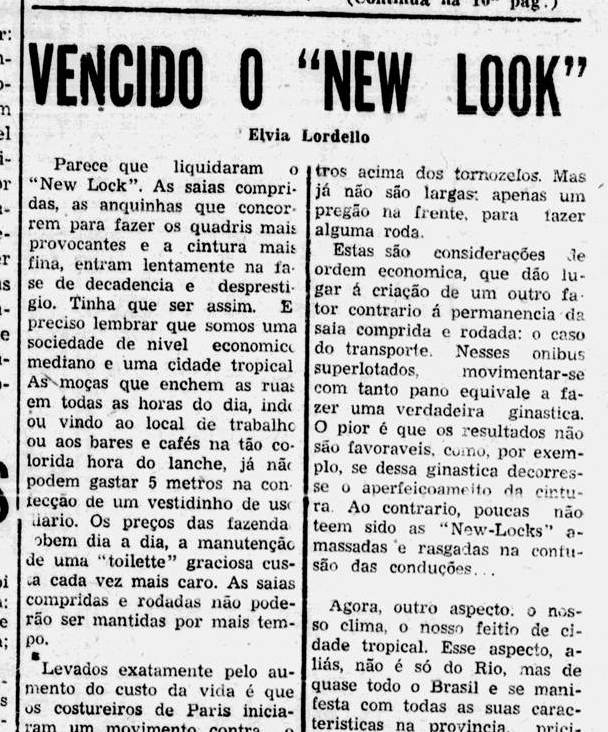
\includegraphics[height=14\baselineskip]{articles/06-vencido-o-new-look-r/03-vencido-new-look.jpg}
        \hspace{\marginparsep}
        \begin{minipage}[b]{\marginparwidth}
            \caption{Artigo ``Vencido o `New Look'{}''.}
            \caption*{Fonte: Biblioteca Nacional, Brasil (Hemeroteca Digital) --- Diário de Natal, ano 1949, ed. 01768, 23 jan. 1949.}
            \label{fig:vencido-new-look}
        \end{minipage}
    \end{wrapfigure}%

    A reportagem apresenta o lançamento do modismo supracitado imerso em um contexto econômico caótico em virtude do pós-guerra. Mesmo assim, não foi empecilho para a ditadura da moda, a qual impôs saias compridas e caras. É que a moda então se baseava no capital, produzindo modelos caros e não se preocupando com a elegância feminina.

    Em 1949, dois anos após a apresentação do \textit{new look}, era publicada uma reportagem intitulada ``Vencido o New Look'' (figura \ref{fig:vencido-new-look}), escrita por Eva Lordello. De acordo com a matéria, o \textit{new look} estava saindo de moda, pois as anquinhas estavam sendo abandonadas junto das saias compridas que davam às mulheres cinturas mais finas, é possível perceber que a repórter ``agradeceu'' por essa moda estar indo embora por dois fatores: a questão econômica, que o Brasil e Natal ocupavam: ``os preços das fazendas sobem dia a dia, a manutenção de uma \textit{`toillete'} graciosa custa cada vez mais caro. As saias compridas e rodadas não poderão ser mantidas por mais tempo''. E as condições tropicais não só do país como da capital, quando argumentou que para o \textit{new look} eram necessários 5 metros de tecido, como moças tropicais e de situação econômica mediana, talvez não conseguissem usar esses vestidos diariamente.

    \textcite{Lordello1949Vencido} ainda argumentava que o modismo estava fora de moda, até mesmo em Paris, pois a tendência requeria muitos metros de tecido: ``tantas saias, tantos babados, tantas rendas e tantas fitas, um Deus nos acuda de accessorios quase inuteis, tirando a graciosidade da silhueta, ou deformando outras de si mesmas, propensas a poucos panos''. Percebe-se a apatia da repórter em relação ao \textit{new look}, no fragmento em questão o qual ela expressava sua insatisfação quando argumentou acerca dos excessos, que acabavam por tornar aquela peça feia, consequentemente a mulher também enfeirar-se-ia. Mediante Lordello, as mulheres queriam sempre o novo, o contemporâneo, e aqueles modelos de Christian Dior já estavam ultrapassados. Em consonância com a overdose estética que o estilista havia lançado dois anos atrás, Loredello continuava suas resistências argumentando que as saias amplas eram empecilhos para o transporte: ``nesses onibus superlotados, movimentar-se com tanto pano equivale-se a fazer uma verdadeira ginastica''; percebe-se a dificuldade até de se movimentar com tal criação extravagante.

    Outro exemplo das críticas a Dior, que esteve presente no jornal, foi a de Bárbara \textcite{Miller1953Luta}. A repórter retratava sobre a resistência das secretárias nova-iorquinas, face à última moda lançada pelo estilista, a saia recém-lançada, que era muito curta: ``'só temos duas mãos: uma para escrever e outra para segurar a saia e cobrir os joelhos''. Nesta matéria, é possível perceber que Dior estava retornando à moda de 1920, com saias mais curtas, com 40 cm do chão, evidenciando que a matéria retratava a resistência feminina não somente ao \textit{new look}, mas a Christian Dior e às suas criações. As novas saias estavam mais curtas, e a jornalista indagava acerca da receptividade, se o estilista conseguiria lançar as saias no mercado e se estas seriam bem aceitas pelas moças, tendo em vista o tamanho das peças.  

    Na mesma reportagem aparece uma ``entrevista'' com Christian Dior, ou ao menos perguntas para o estilista, sobre as críticas que estava recebendo. Assim, questionado sobre a inovação estética, o costureiro disse que se vivia uma nova era. A resistência foi sentida não apenas pelas natalenses, mas por outros modistas (não foi informado se eram de Paris ou de outros lugares), que se mostraram apáticos à criação do francês. Como as críticas direcionavam-se às saias curtas, a reportagem acreditava que essa moda não pegaria, sobretudo pelas secretárias de Nova York para quem as novas peças atrapalhavam o trabalho.  

    Portanto, as tramas do sistema da moda, durante os anos de 1948--53, estavam desfavoráveis não somente ao \textit{new look}, criação de Christian Dior, mas ao estilista e também às modas por ele produzidas. Estas resistências serão apresentadas outras, ainda que dialoguem diretamente com o \textit{new look}, mas que não receberam dos jornais a expressão ``new look'', podemos inferir que trata-se do modismo criado pelo francês, pelas características principalmente das saias rodadas. Neste sentido, soma-se à tessitura do texto em questão, as apropriações das moças, presentes principalmente na seção ``Notícias da Moda'', entre os anos de 1948--1950, bem como as reportagens que retrataram os conflitos entre saias mais curtas e/ou mais compridas. Assim, pode-se inferir que as novas modas, de saias de comprimento reduzido, e as mais alongadas também receberam influências diretas das criações de Dior.  

    A partir das reportagens analisadas, percebe-se que entrava em conflito os gostos e os discursos jornalísticos, para tanto, Calanca acerca do gosto, diz que: ``o gosto, portanto, define-se como faculdade de julgar desinteressadamente um objeto ou uma representação mediante um prazer ou um desprazer'' \cite[p.~93]{Calanca2008Historia}. A partir de Calanca, identifica-se que os embates no tocante ao \textit{new look} em Natal, perpassaram o gosto, das que escreviam as matérias jornalísticas, mas também das moças que faziam o uso do estilo, logo, infere-se que o gosto pelo \textit{new look} variava entre as jornalistas que resistiam e reprovavam a tendência e, sobretudo, as natalenses que adotaram tal moda. Em consonância, insere-se na discussão, o conceito de gosto, amplamente utilizado por Medeiros Filho, quando compreende que as moças em São João do Sabugi não vestiram diretamente o \textit{new look}, mas o arremedaram mediante as suas condições (climáticas, econômicas, culturais).

    \section{Notícias da Moda, uma seção de modos e modas}

    \nocite{NoticiasDaModa1948janeiro}

    Durante os anos de 1948--50 no \textit{Diário de Natal}, as moças que quisessem se informar sobre as efemeridades da moda leriam a seção ``Notícias da Moda'', na página feminina do periódico. Por entre as páginas da seção de modos e modas, as moças atualizar-se-iam acerca das tendências, dos desfiles estrangeiros, dos comprimentos das saias e os conflitos que estes tamanhos ocasionariam. Neste sentido, ainda que os jornais silenciem, nas suas páginas percebeu-se que tal seção vigorou apenas por três anos, pois após 1950 as reportagens sobre moda não apareceram mais naquela coluna, mas dispersas no periódico.

    Outrossim, a seção supracitada servia apenas como informativo no tocante aos modismos e novidades estrangeiras que aportavam em Natal, mas de formadora de opinião sobre o que as moças deveriam vestir. Definia-se o que era considerado atual, os usos que seriam apropriados, as resistências mediante os parâmetros morais e estéticos, se cobririam e se embelezariam a partir das silhuetas retas e esguias ou das amplas e rodadas saias. Pelas páginas, foi possível identificar que o conflito entre o comprimento das saias estava imerso também quando Christian Dior lançou o \textit{new look} o que estendeu as resistências ao estilista e não somente à sua clássica e revolucionária criação. 

    Nas primeiras ocorrências que retratavam sobre as saias curtas e compridas, ainda em 1948, é possível inferir que a dúvida instaurada acerca dos comprimentos, fazia-se presente entre os cortes masculinizados e retilíneos, sem muitas curvas, formando uma silhueta séria e sóbria, ou mais cortes afeminados, enaltecendo a feminilidade, através de ancas, drapeados e saias rodadas. Tais tendências eram importadas de Paris, e ainda que advindas da capital da moda, não agradavam a todos, sobretudo pelo tamanho das saias, mais curtas, pouco abaixo do joelho. Para além das saias, outra tendência que estava acarretando reprovações estéticas era o uso de calças inspiradas nas \textit{maisons} Balmain, Hermés, Lanvin, que apresentavam calças para as mulheres como símbolo de modernidade.

    Tais frivolidades da moda, que desagradavam tantos, eram como as estranhezas do tempo da guerra, com os cortes totalmente diferentes, não eram mais masculinizados e sim com pregas e drapeados, como mostra a reportagem da seção abordada no tópico em questão: ``as prezas, os drapeados são os característicos dessa tendência suntuosa.'' Por meio do fragmento da reportagem, é possível perceber que as novidades eram opostas àqueles que preferiam a simplicidade dos trajes, da silhueta sisuda, evidenciando que a moda não estava sendo bem aceita por todos, pois os novos padrões eram totalmente diferentes dos anteriores, uma verdadeira revolução estética.  

    As tentativas em resgatar o comprimento das saias mais compridas não estavam vigorando, pois era inconveniente para o ano de 1948. Logo, apesar de opostas às saias longas e armadas, o jornal mostrava que as moças não deveriam fazer o uso de saias muito curtas. Entretanto, ``não nos referimos é claro, aos vestidos demasiadamente curtos com que certas senhoras de fartas carnes e de não menos avultadas banhas timbram em usar, dando assim uma demonstração eloquente de falta de tato e de equilíbrio.'' Através do fragmento da reportagem, percebeu-se que, de acordo com o \textit{Diário de Natal}, as mulheres não deveriam usar grandes e compridas saias, tampouco saias muito curtas, que exibissem demais suas fartas carnes. Pela concepção do periódico, o comprimento ideal seria pouco abaixo do joelho, visto que estas saias eram mais confortáveis, e ideais para mulheres que precisavam trabalhar fora de casa, pois não eram complicadas de se movimentarem, além de diferenciarem dos homens já que não eram tão parecidas com as vestes masculinas. É perceptível que o jornal também se colocava no papel de ditar a opinião pública, como o caso de formar o imaginário feminino acerca das roupas mais adequadas para sair de casa e para trabalhar. 

    Ainda sobre a extensão das saias, e em consonância com o corpo feminino, Rosa \textcite{Kaliweyer1948Batalha} em ``A batalha das modas da primavera em Paris'', retratou que ``a linha apresenta-se esguia. A cintura fina e flexível. O busto redondo e alto''. As formas femininas deveriam ser, deste modo, a partir da reportagem, finas com bustos que destacassem os seios e os elevassem. Para além dessas características, na mesma reportagem, Kaliweywer ressaltava que imperava entre as mulheres o uso de saias rodadas, mesmo que algumas usassem as saias mais justas ao corpo, as \textit{godets}\footnote{\textcite{MedeirosFl2014Arremedando} compreende as saias godês, ou \textit{godets}, enquanto fragmentos triangulares do tecido das saias o que as torna mais largas e dão o efeito de saia rodada.} se sobressaíam, percebe-se assim que as resistências a Christian Dior e às suas modas não eram totalmente aplicadas, pois uma de suas criações e disseminações foram as saias \textit{godets}, que segundo a reportagem em questão estavam sendo amplamente apropriadas ``apesar de se verem muitos modelos com saias estreitas, as rodadas predominam e oferecem maior variedade.''\footnote{Ibidem.} Por meio dos amplos usos, o mercado era mais variado para as \textit{godets}.

    Atrelada às saias \textit{godets}, Kaliweyer argumentava que as pregas, pinças e franzidos se combinavam com muitos babados e tecidos, confeccionadas em tafetá, \textit{mousselines}\footnote{Segundo \textcite{MedeirosFl2014Arremedando}, \textit{mousselines} corresponde à tecidos frágeis, utilizados para a feitura de indumentárias íntimas.}, rendas e bordados, em tons pastel de azul e rosa, na reportagem aparece menção às saias que encurtaram em 25 centímetros. É nítida as relações diretas com o modelo de Christian Dior, refletidas nas pregas, rendas, babados assim como no tamanho da saia.

    \nocite{CurtasOuCompridas1948}
    \nocite{NoticiasDaModa1948janeiro}
    \nocite{NoticiasDaModa1948Junho}
    \nocite{DiarioDeNatal1949SemTitulo}

    Em consonância com as noções de saias mais curtas ou compridas, uma reportagem da seção ``Notícias da Moda'', retratava que a moda em 1949 estava sendo diferente das anteriores em virtude das resistências, logo, encontravam-se mulheres com saias rodadas e saias retas, estas últimas não haviam se adaptado ou rendido à moda das primeiras: ``E com os `panneaus'\footnote{Termo em francês que foi usado para referir-se a tecido leve, no caso da reportagem os tecidos das saias.} soltos, drapeados, plissados, notas embelezadouras da silhueta estreita; com a ampliação da saia leva para traz, o que no tailleur, o casaco repete.'' Pode-se perceber que a tendência das pregas estava sendo a preferida entre as mulheres, presentes também nos casacos, sobretudo entre os tailleurs, os quais contrastavam com as saias estreitas. 

    Face ao caráter cíclico da moda, o periódico tratava o retorno à moda dos vestidos com o comprimento abaixo do joelho, onde as mulheres o trajavam exibindo elegância, sobretudo quando eram usados de noite, as saias eram rodadas e estampadas, combinados com um corpete que ajudava na modelação do corpo, os quais tinham Paris como maior centro de referência para a moda brasileira e, no caso de Natal, os arremedos franceses que a capital potiguar fazia em relação à capital francesa. Percebe-se ainda que a moda das saias rodadas ainda imperava, principalmente para as moças irem para os bailes noturnos, a silhueta estava em transformação, transformação que não é especificada pelo jornal. 

    As saias longas não vigoraram por tanto tempo. No começo assim que essas surgiram foram criticadas pelo tanto de pano que necessitavam, impossibilitando os movimentos femininos, os vestidos grandes foram tão revolucionários, pois transformaram a ordem estética vigente por dez anos, que era das saias curtas. Com a Segunda Guerra o cenário indumentário transfigurou-se, visto que o estilista Christian Dior substituiu a masculinidade dos trajes femininos, muito presentes na década de 1940, com o conflito armado tal situação mudou com a volta das saias curtas, assim, ainda que as mulheres não estivessem animadas com a moda, o inverno de 1949, estava chegando e as mulheres precisavam de roupas da moda, moda essa que havia ampliado as possibilidades de saias, \textit{godets}, rodadas, com pregas, lisas, estampadas. 

    As modas estrangeiras eram de vestidos mais compridos, mas quando estes chegavam no Brasil eram arremedados e diminuído, um exemplo das efemeridades e arremedos, como explicitado no fragmento a seguir:

    \begin{quotation}
        O tempo das saias compridas morreu com a falências de certas teorias retrógradas que limitavam á mulher todas as suas possibilidades e aspirações e, compreendendo isso, assim como sendo a aceitação sem raciocínio, de todas as imposições da moda, o índice de uma mentalidade de que elas, de possuídas, ao analisarem por todos os prismas da moda da saia comprida, resolveram protestar, conservando os seus vestidos sincrónicos com a vida dinamica e liberta de certos preconceitos retrógrados que caracterizam nossos dias.
    \end{quotation}

    Pode-se inferir a partir do fragmento de reportagem que as saias compridas eram opressoras das mulheres e dos seus movimentos. Já o abandono de tal tendência e adoção de saias mais curtas poderia significar o abandono de tais opressões que limitavam os movimentos.

    \section{Alguns retoques finais}

    À guisa de conclusão, em função do exposto, compreende-se que as resistências ao new look foram importadas da Europa, dos Estados Unidos, e de outras localidades do Brasil como o Rio de Janeiro, e terminaram por desembocar em Natal, influenciando as leitoras do \textit{Diário de Natal} a se vestirem, comportarem, recusarem e aceitarem certas tendências. Além de tal concepção, é possível argumentar que as resistências ocorreram ao passo de que as apropriações também estiveram presentes na sociedade natalense, pois pelas reportagens foi possível identificar tais conflitos entre as moças que eram contrárias e as que eram favoráveis ao modismo.

    O estilista e costureiro francês Christian Dior foi o principal alvo das críticas e resistências das matérias analisadas na presente exposição pelos seguintes motivos: demanda de muitos metros de tecido para a confecção das amplas e rodadas saias, dificuldade de se movimentar, problemas no transporte público, clima inadequado para o novo modismo. Ainda assim, com tais manifestações avessas a Dior, o estilista consagrou-se no mercado de alta-costura francesa, influenciando o mercado da moda mundial com a combinação de saias \textit{godets}, e \textit{tailleur}. Os escritos acerca da moda eram registrados, sobretudo entre 1948--1950 na seção ``Notícias da Moda'', que era responsável por formar o pensamento relacionado aos novos cortes e silhuetas bem como intervir no cotidiano potiguar.  

    Logo, a história que aqui foi retratada pelo periódico proporciona a compreensão de outras histórias do Rio Grande do Norte, não somente calcadas nos jogos políticos das oligarquias, mas também numa história pelas tramas dos costumes, das costuras, das tendências e efemeridades, evidenciando a necessidade de se conhecer, pesquisar e estudar sobre os discursos da moda, suas possibilidades, e neste caso em específico, as resistências.

    \printbibliography[heading=subbibliography,notcategory=fullcited]

    \hfill Recebido em 15 abr. 2021.

    \hfill Aprovado em 19 abr. 2021.

    \label{chap:vencidonewlookend}

\end{refsection}
